\subsection{Evaluation Overview}
\label{sec:evaluationoverview}

% main picture of the overview of the system for evaluating the esb and explain it with detais of the hardware setup of the vm
% describe a little bit the scenarios that were fixed
% 
In the Section \ref{sec:requirements} we have described the requirements that the evaluation should fulfill and the needed modifications in the utilized benchmark. As exposed in Figure \ref{fig:evaluationoverview}, the evaluation is conformed by three main independent systems. We must ensure, for analyzable purposes, that we approximate as much as possible to a Web service standard real scenario: service requester invokes a backend service and both request and response are routed through the network. In our evaluation we must utilize the \ac{ESB} as a mediator between the service requester and provider. In the first system (VM0), both service requestor and provider are deployed. The communication measurements are taken in two different components: throughput and response time in the AndroitLogic driver, while the number of incoming and outgoing requests, as well as the visualization of the messages, have to be monitored in an independent monitoring component. 

In the second and third systems (VM1 and VM2 respectively) one instance of ServiceMix is deployed for routing the messages between the AndroitLogic driver and the backend service. A monitor component must perform the counting of the incomming and outgoing requests to and from the \ac{ESB}, and a system monitor component should measure the \ac{ESB}'s resources consumption. The connection between the components in VM0 and VM2 is represented with a dashed line, because the VM2 is only use for non multi-tenant aware scenarios. Similarly, we have connected the components in VM0 with the components in VM1 with a continuos line, because this connection is used in both multi-tenant and non multi-tenant aware scenarios. 

The JBIMulti2 application is used for deployment of the \ac{SA}s which pack the endpoint configurations in the \ac{SU}s. However, we do not include the JBIMulti2 application in our overview because we do not evaluate the JBIMulti2 performance, but the multi-tenant and non multi-tenant ServiceMix independently from the JBIMulti2 application.

\begin{figure}[htb]
	\centering
		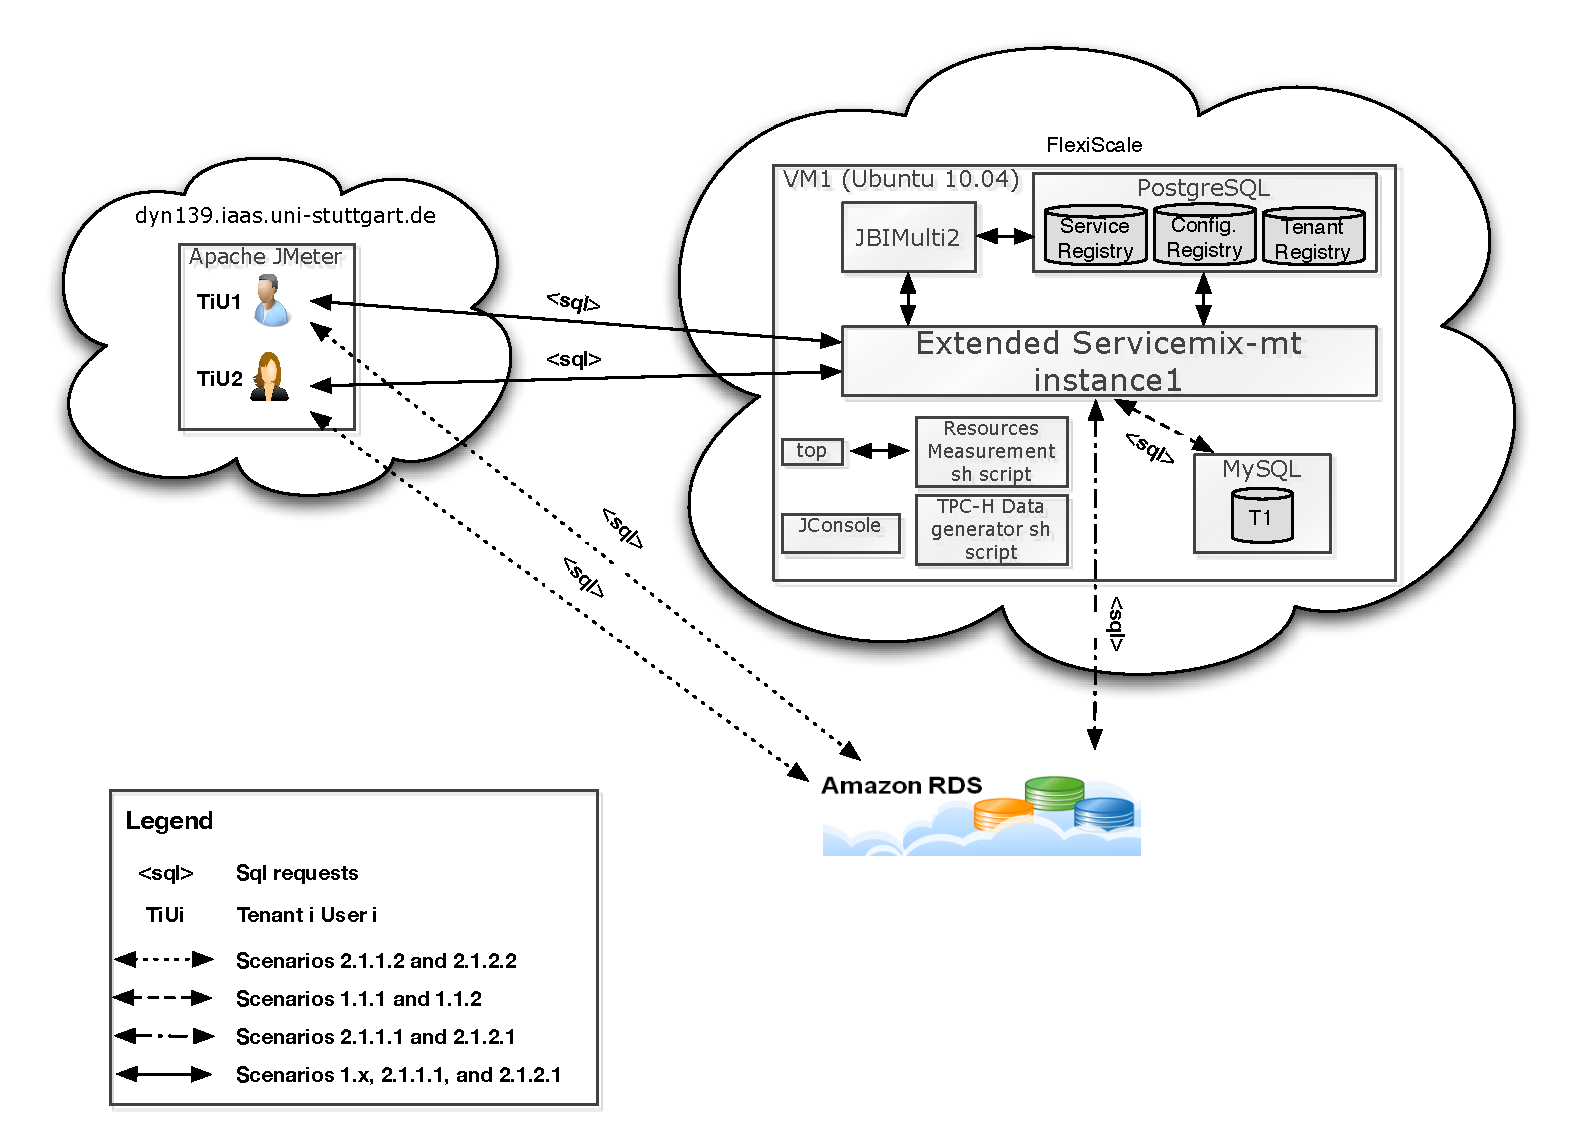
\includegraphics[width=0.7\textwidth, trim=0.0cm 0.0cm 0.0cm 0.0cm, clip]{./gfx/evaluationoverview.pdf}
	\caption[Performance Evaluation Components Overview]{Overview of the components used for the \ac{ESB} performance evaluation. \textbf{Note:} In the evaluation two different monitors are used. For communication the monitoring requires the counting and visualization of the incoming and outgoing requests. For system monitoring, the CPU and Memory usage should be measured.}
	\label{fig:evaluationoverview}
\end{figure}

\FloatBarrier